%http://www.electronics.oulu.fi/latex/examples/example_1/
%\documentclass{article}
\documentclass[12pt,epsfig]{article} 
%\documentclass[12pt,epsfig]{report} %CLAS analysis note 
% If [12pt,epsfig] is not put along side the documentclass, the '=' sign shows
%    up as a '-' inside 'equation' or 'eqnarray'

\usepackage{lineno}
%\usepackage{graphicx}
\usepackage[dvips]{graphicx} 
\usepackage{rotating}
\usepackage[usenames]{color} 
%\usepackage[dvips]{color}  %kp: added  %http://www.eng.cam.ac.uk/help/tpl/textprocessing/latex_advanced/node13.html
\usepackage[usenames]{xcolor} %kp: http://tex.stackexchange.com/questions/25538/colors-known-to-pdf
\usepackage{epsfig}
\usepackage{url}
\usepackage{float}
\usepackage{verbatim}
\newcommand\numberthis{\addtocounter{equation}{1}\tag{\theequation}}
\usepackage{pst-plot}
\usepackage[breaklinks=true]{hyperref}
\usepackage{bm}
\usepackage{amssymb, amsmath}
\usepackage[numbers,sort&compress]{natbib}
\usepackage{url} 
\usepackage{pst-plot}
\usepackage[font=small,format=plain,labelfont=bf,up, justification=justified]{caption}
\usepackage[section]{placeins} %For \FloatBarrier <= https://en.wikibooks.org/wiki/LaTeX/Floats,_Figures_and_Captions#Tables
\renewcommand{\textfraction}{0.05}
\renewcommand{\topfraction}{0.95}
\renewcommand{\bottomfraction}{0.95}
\renewcommand{\floatpagefraction}{0.35}
\setcounter{totalnumber}{5}

\usepackage{longtable} % nate
\usepackage{appendix} %http://www.tex.ac.uk/FAQ-appendix.html


%kp: 10/24/16: ============ My definitions/shortcuts
\def\t0{$T_0$ }
\def\tmax{$T_{max}$ }





\begin{document}

\title{Calibration of CLAS12 Drift Chambers}
\author{Krishna Adhikari, Mac Mestayer}

\maketitle

\begin{abstract}
In this document the process of DC calibration, mainly the calibration of the time-to-distance function is described. Additionally, the GUI for the calibration suite which is written in Java using CLAS12 common tools is described.
\end{abstract}

%https://texblog.org/2013/04/29/latex-table-of-contents-list-of-figurestables-and-some-customizations/
\tableofcontents
%\listoffigures
%\listoftables

\pagebreak



\section{Introduction}
\FloatBarrier

Drift chambers are used to track charged particles. One can simply do the hit-based tracking in which one simply uses the positions of the hit wires to fit tracks, by ignoring any information regarding the timing of the signals measured for each hit wire. But, to get better resolution, one uses time-based tracking in which timing of the signals is also considered. The raw data from the drift chambers are in the form of TDC digits which can be converted to nano-seconds as measured times of the signals picked by various sense wires of the chambers. These times, in turn, can be converted to drift times of the ions received by the corresponding wires by correcting them for various delays such as the signal propagation delay due to cable lengths, sense wire-lengths and due to flight times of the particles that are used to trigger the events as well as the flight time of the particle being tracked. After the various delays are subtracted off the total measured time, one needs to convert these `true' drift times into corresponding distances also known as DOCAs (distances of closest approach) of the passing tracks from the corresponding sense wires, before they can be used for the track-fitting. This conversion is possible only if one knows the relationship between the measured drift-times and the drift-distances. Since, the relationship depends on various factors such as the type of the drift gas, its temperature and pressure, the strength of the electric field and magnetic fields present, and also on the angle of the tracks (because of the hexagonal geometry of the drift-cells), the mathematical relationship is not a simple and well known expression. Rather, it has to be determined by fitting a certain trial form (based on known physics of ionization and drift) of the function to the actual data coming from the chambers themselves. In this document, the process of determining this `time-to-distance' function as well as the java-based GUI that has been written for this purpose is described. In our case, we actually determine from data-fits a reverse relation of `distance-to-time', which will then be numerically inverted and used by the reconstruction software.



\section{Fit Equations}
\label{sFitEquations}

The trial form of the distance-to-time function that we use is shown in Eq. \ref{timeAll}. 
There are 10 free parameters that should be determined from the fits. Five of them (first four and the last one) are generic, but the other five are B-field dependent (thus applicable only to the region-3 chambers i.e. third and fourth superlayer).

\begin{equation}
\label{freePars}
\begin{aligned}
  p_0 & = v_0 \\
  p_1 & = deltamn = m - n  \\ %In the CCDB table and codes it was initially wrongly named as deltnam and has been kept that way.
  p_2 & = t_{max}   \\
  p_3 & = distbeta = x_{\beta} \\ 
  p_4 & = delta\_bfield\_coefficient = \delta_{B} \\
  p_5 & = b_1  \\
  p_6 & = b_2  \\
  p_7 & = b_3  \\
  p_8 & = b_4 \\
  p_9 & = \Delta T0
\end{aligned}
\end{equation}

(The last parameter was added later as an additional correction to the time-delay correction T0.)

The overall equation for drift time 't' is:

\begin{equation}
\label{timeAll}
\begin{aligned}
     t = \frac{x}{v_0} + a \cdot \hat{x}^n + b_{\alpha}\cdot \hat{x}^m + \Delta t_{B} + \Delta t_{\beta}
     %time = \frac{x}{p_0} + \hat{x}^n + \hat{x}^m + \Delta t_{B} + \Delta t_{\beta}
     %To keep the inflection point behaviour 'b_alpha' is always -ve and m>n
\end{aligned}
\end{equation}

with $\hat{x} = x / x_{max}$ and last two terms given by the following expressions:

\begin{equation}
\label{Delta_t_B}
\begin{aligned}
  %\Delta t_{B} = delta\_bfield\_coefficient \cdot B^2 \cdot t_{max} \cdot
  \Delta t_{B} = \delta_{B} \cdot B^2 \cdot t_{max} \cdot
            (b_1 \hat{x_{\alpha}} + b_2 \hat{x_{\alpha}}^2 + b_3 \hat{x_{\alpha}}^3 + b_4 \hat{x_{\alpha}}^4  )
\end{aligned}
\end{equation}

\begin{equation}
\label{Delta_t_beta}
\begin{aligned}
     %\Delta t_{\beta} = \frac{ \sqrt{x^2 + (distbeta \cdot \beta^2)^2} - x }{ v_0 }
     \Delta t_{\beta} = \frac{ \sqrt{x^2 + (x_{\beta} \cdot \beta^2)^2} - x }{ v_0 }
     %\Delta t_{\beta} = \frac{ \sqrt{x^2 + (p_3 \cdot \beta^2)^2} - x }{ p_0 }
\end{aligned}
\end{equation}

Due to the constraints described in the section that follows, the coefficients `a' and `b' and the exponents `m' and `n' are correlated and, therefore, we can reduce the number of free parameters to be determined from the fits. That is the reason why we see `a', `b', `m' and `n' don't show up as free parameters in the equation \ref{freePars} above.


\subsection{Constraints of the equation}
\label{constraintsTvsX}
For 30 degree tracks (and in the absence of B-field such as in regions 1 and 3): \\
The first constraint is that $t = t_{max}$ when $x = d_{max}$, which results in the following equation:

\begin{equation}
\label{tvsxConstraints1}
\begin{aligned}     
     t_{max} = \frac{d_{max}}{v_0} + a + b
  \end{aligned}
\end{equation}

The second constraint is that the drift velocity $dx/dt = v$ at $x=0$ is equal to that at $x=d_{max}$ (and thus both equal to $v_0$ because the former is closest to the sense wire(s) and the latter is closest to the field wires and in the nearest vicinity of each, the electric field is very high so that the ions reach the saturated velocity of $v_0$. This constraint, results in the following relationship:

\begin{equation}
\label{tvsxConstraints2}
\begin{aligned}     
     a = - b \frac{m}{n}
  \end{aligned}
\end{equation}

Finally, the third constraint is that an inflection point (a minimum in velocity) occurs at a certain distance between $x=0$ and $x=d_{max}$, because the as one moves away from the sense wire the field gradually decreases and reaches a minimum and then it starts to grow again as it moves closer to the field wire. Mathematically, the inflection point is defined as the point where the second derivative of `x' i.e. drift acceleration becomes zero. From past studies using GARFIELD simulations (contact M. Mestayer about this), the inflection point has been determined to occur at $x = 0.615\cdot d_{max}$. As a result, the following relationship is arrived at:

\begin{equation}
\label{tvsxConstraints3}
\begin{aligned}     
     n =  \frac{1 + (deltamn - 1) 0.615^{deltamn}}{ 1 - 0.615^{deltamn}}
  \end{aligned}
\end{equation}





\subsection{Initial best guess (nominal) values of the parameters}
Based on past experiences and GARFIELD studies, we started with the following best guesses (see Table \ref{tParInitialValues}) of the values for the parameters of the time-to-distance function:


\begin{table}[H]
\centering
\begin{tabular}{l*{6}{c}r}

Parameter   Names       & Initial best guesses \\
\hline
  $p_0$    &  $v_0$                   & 0.0047 cm/s   \\
  $p_1$    & $deltamn$            & 1.5   \\
  $p_2$    & $t_{max}$            & tMaxSL    \\
  $p_3$   & $distbeta$            & 0.05  \\ 
  $p_4$    & $delta\_bfield\_coefficient$    & 0.16  \\
  $p_5$    & $b_1$                     & 0.4  \\
  $p_6$    & $b_2$                     & -2.0 \\
  $p_7$    & $b_3$                     & 10.0 \\
  $p_8$    & $b_4$                     & -6.5  \\
  $p_9$    & $\Delta T0$             & 0.0 \\
\hline
\end{tabular}
\caption{Initial (nominal) values of the parameters of the time-to-distance function. Here, tMaxSL = 165, 175, 300, 320, 525 and 550 ns respectively for the six different superlayers SL1, SL2, SL3, SL4, SL5 and SL6.}  
\label{tParInitialValues}
\end{table}



%#################################
\section{Procedure}
\label{lProcedure}

First of all, the good hits associated with well reconstructed tracks (from time-based tracking) are selected from each event. The corresponding segment from the TBSegments bank are identified and the local angles of these segments are used to define the 
angular bins into which these hits are divided. In each of these bins, we make a two-dimensional histogram (see Fig. \ref{fTimeVsTrkDoca} for an example) of the T0 corrected 'time' and 'trkDoca' variables of the hits thus selected. In the case of hits from superlayers 3 and 4, where the torus magnetic field is present, we further divide data into bins of B-field. Since the binnings in the local angle ($\alpha$) and magnetic field ($B$) are reasonably small enough in size (or width), we assign an average value of angle and B-field to all the hits beloing to that particular bin and these average values will be used during the $\chi^2$-minimization process that we employ to determine the parameters of the time-to-distance function.


\begin{figure}
    \centering
    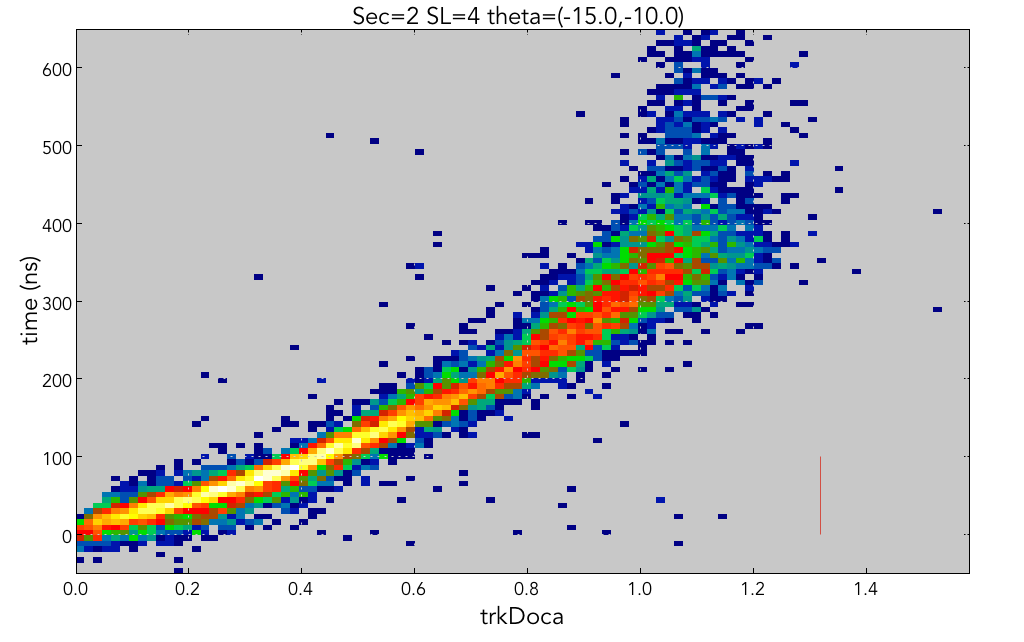
\includegraphics[width=1.0\textwidth]{Figures/time_vs_trkDocaExample_Sec2_SL4_th_m15_m10.png}
    \caption{An example of the time-vs-trkDoca 2D histogram in a given bin (-15,-10) of local angle $\alpha$.}
    \label{fTimeVsTrkDoca}
\end{figure}


These 2D-histograms are then transformed into X-profiles (see Fig. \ref{fTimeVsTrkDocaXProfile} for an example)  which are essentially GraphError objects with each data point made out of the average value and error of the Y-variable ('time' in our case) distribution corresponding to a particular bin of X-variable (trkDoca in our case). And, the data points of these profiles are what we use in the $\chi^2$-minimization procedure using \href{http://java.freehep.org/freehep-jminuit/}{jMinuit} (\href{http://java.freehep.org/}{FreeHEP} Java implementation of the Minuit library) which has been included in the CLAS12 common tools package known as COATJAVA.

\begin{figure}
    \centering
    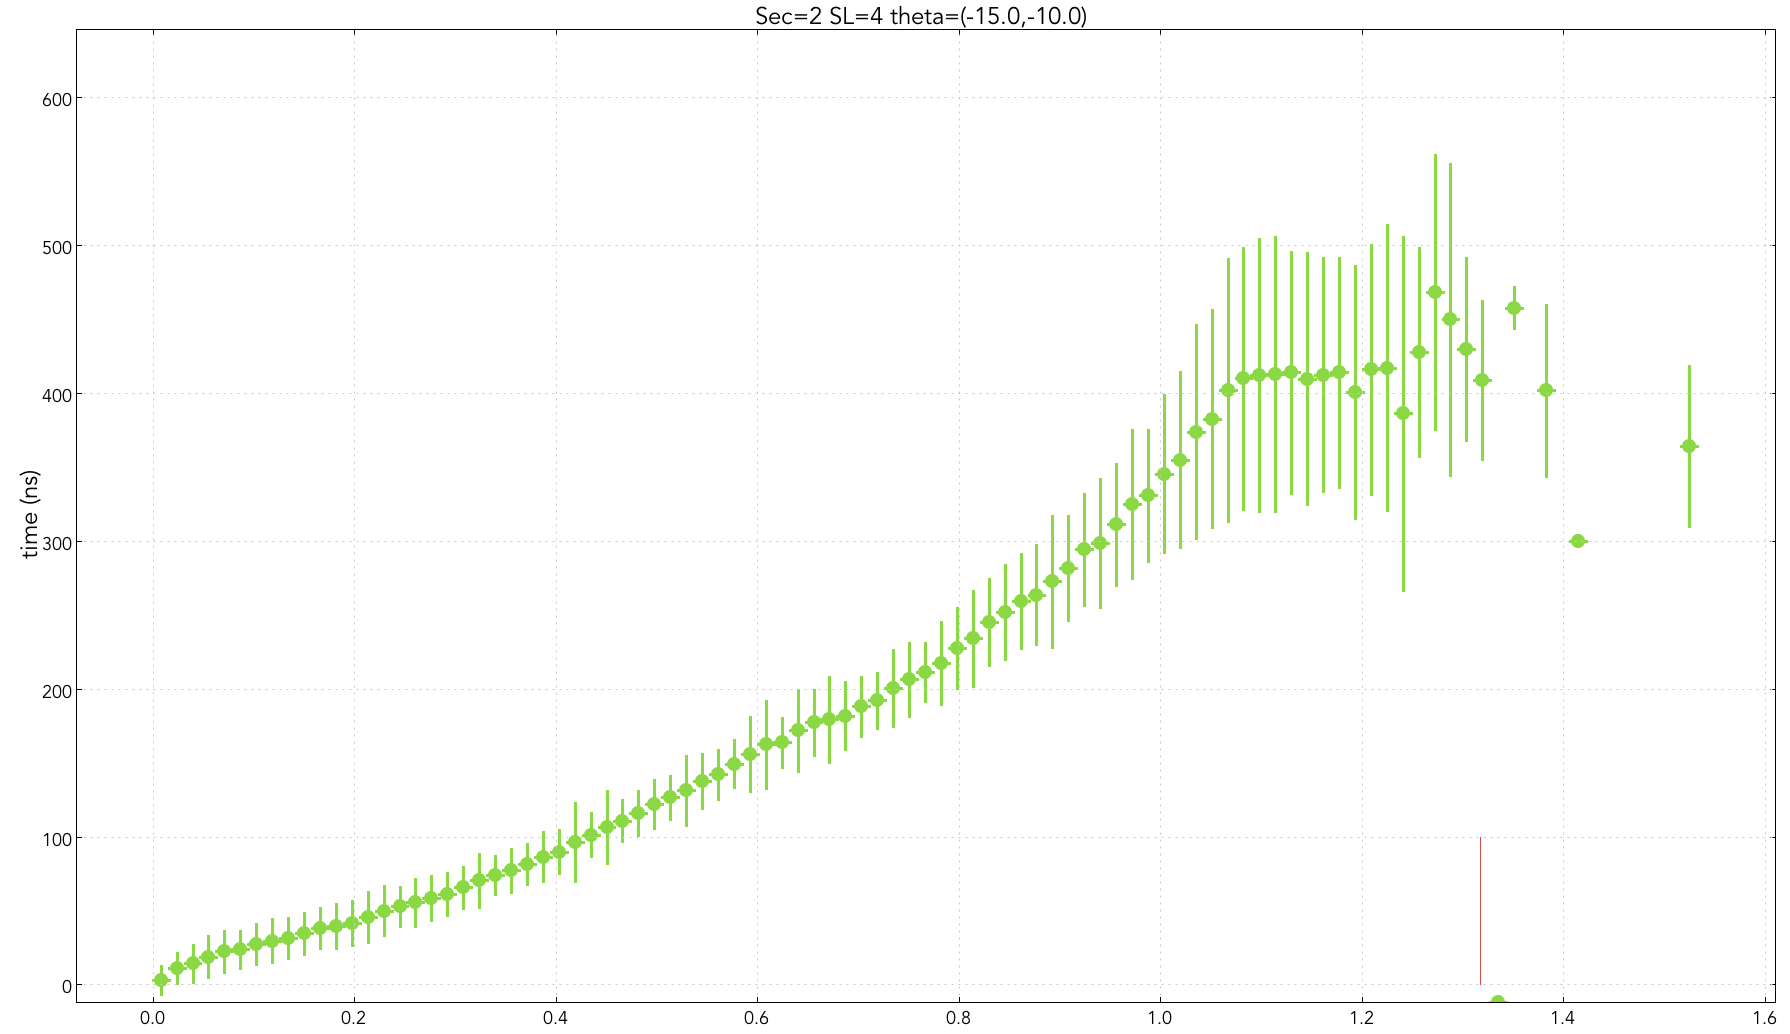
\includegraphics[width=1.0\textwidth]{Figures/time_vs_trkDocaXProfileExample_Sec2_SL4_th_m15_m10.png}
    \caption{An example of the X-profile of  the time-vs-trkDoca 2D histogram in a given bin (-15,-10) of local angle $\alpha$.}
    \label{fTimeVsTrkDocaXProfile}
\end{figure}


\subsection{Data Binning}

Currently, the data is grouped into 17 local angle ($\alpha$) bins as listed in the table \ref{tAngleBins}. Out of the 17 bins, only the selected few (fourth, fifth, sixth, tenth, eleventh and twelfth)  bins have been used for the simultaneous fits. Because the resolution gets worse for tracks with local angles close to zero and 30 degrees, the data from the bins closer to zero degree, or 30 degree and beyond have are skipped in the fitting procedure. The bin selection can now be done by opening the 'Bin-selector' panel from the fit-control panel of the calibration package. So, if we decide to chose different bins in order to use in the fitting procedure, we can simply do that by clicking on the check buttons for the corresponding bins in the bin-selector panel.

\begin{table}%[H]
\centering
\begin{tabular}{l*{6}{c}r}

Bin         & Minimum    & Maximum   & Average\\
\hline
0                 & -55.0    &  -45.0     \\
1                 & -45.0    &  -35.0     \\
2                 & -35.0    &  -25.0     \\
3                 & -25.0    &  -20.0     \\
4                 & -20.0    &  -15.0     \\
5                 & -15.0    &  -10.0     \\
6                 & -10.0    &  -6.0       \\
7                 & -6.0      &  -2.0       \\
8                 & -2.0      &   2.0       \\
9                 &  2.0      &   6.0       \\
10               &  6.0      &   10.0     \\
11               &  10.0    &  15.0       \\
12               &  15.0    &  20.0       \\
13               &  20.0    &  25.0       \\
14               &  25.0    &  35.0       \\
15               &  35.0    &  45.0       \\
16               &  45.0    &   55.0       \\

\hline
\end{tabular}
\caption{Binnings used for the local angle $\alpha$.}   \label{tabParLimits}
\label{tAngleBins}
\end{table}

Similarly, we also have to choose binnings for the magnetic field B (bin-selector panel for the B-field is yet to be adde). Currently, the B-field distribution in data belonging to KPP run 810 extends only up to about 1.2 Tesla as shown in the Fig. \ref{fBfieldDist}. And, for convenience for now, only one slice (bin) of B-field distribution in the range (0.4,0.6) T has been used for superlayers 3 and 4. Later, capability to chose more bins will be added (just like for the local angle bins) by adding one more bin-selector panel to choose the B-field bins.

\begin{figure}
    \centering
    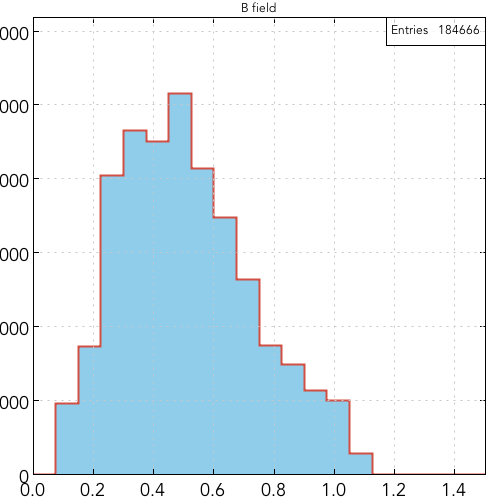
\includegraphics[width=1.0\textwidth]{Figures/bField_KPP_Run810.png}
    \caption{Distribution of B-field in the data for KPP run 810.}
    \label{fBfieldDist}
\end{figure}




\subsection{Evaluation of $\chi^2$ to be Minimized}
\label{ssChisqEval}
The $\chi^2$ that is passed to the jMinuit for minimization in order to optimize the values of the free parameters is calculated by making a sum over all X-profile data points:

\begin{equation}
\label{eqChiSq}
\begin{aligned}
  \sum_{all-good-hits}^{}  \Bigg(   \frac{t_{meas} - t_{calc}}{ \Delta t} \Bigg)^2
\end{aligned}
\end{equation}

In Eq. \ref{eqChiSq}, $t_{meas}$ is the Y-coordinate of a data point from the X-profile, which is essentially the average (in a given X-slice) of measured times (TDC readings) after correcting for various time delays (read from the `time' variable in TBHits bank in the data file). On the other hand, $t_{calc}$ is the time calculated using the distance-to-time function using the corresponding `trkDoca'  value read from the TBHits bank and the trial set of time-to-distance parameters (passed by Minuit). The difference of the two times is weighed by the factor $1/\Delta t$, where $\Delta t$ is the uncertainty in the calculation of average-time of each data point of the X-profile. Currently, three options have been tried for $\Delta t$ - (a) giving it a value of 1.0, which is essentially giving an equal weight to each of the X-profile data points no matter what the statistic was in each of the X-slices, (b) giving it a value of RMS (root-mean-square) of the time-distribution in the corresponding X-slice, and (c) giving it a value of $\sqrt{N}$, where `N' is the number of counts in a given X-slice.

Once the $\chi^2$ is calculated using all the X-profile data points (one can discard some X-profile data points that fall outside of a selected range in `trkDoca' (using the `xNormMin' and `xNormMax' fields in the fit-conrol panel (see Sec. \ref{ssFitControlPanel}) ) from selected bins of local angle and B-field, it is passed to the Minuit for a simultaneous fit by the method of $\chi^2$-minimization and in the end it will return some optimum values of the free parameters, which will then be used to to make the fit lines to plot on top of the corresponding `time-vs-trkDoca' and `X-profile' plots as shown in Figs. \ref{fTimeVsTrkDocaWithFit} and \ref{fTimeVsTrkDocaXProfileWithFit}.
\begin{figure}
    \centering
    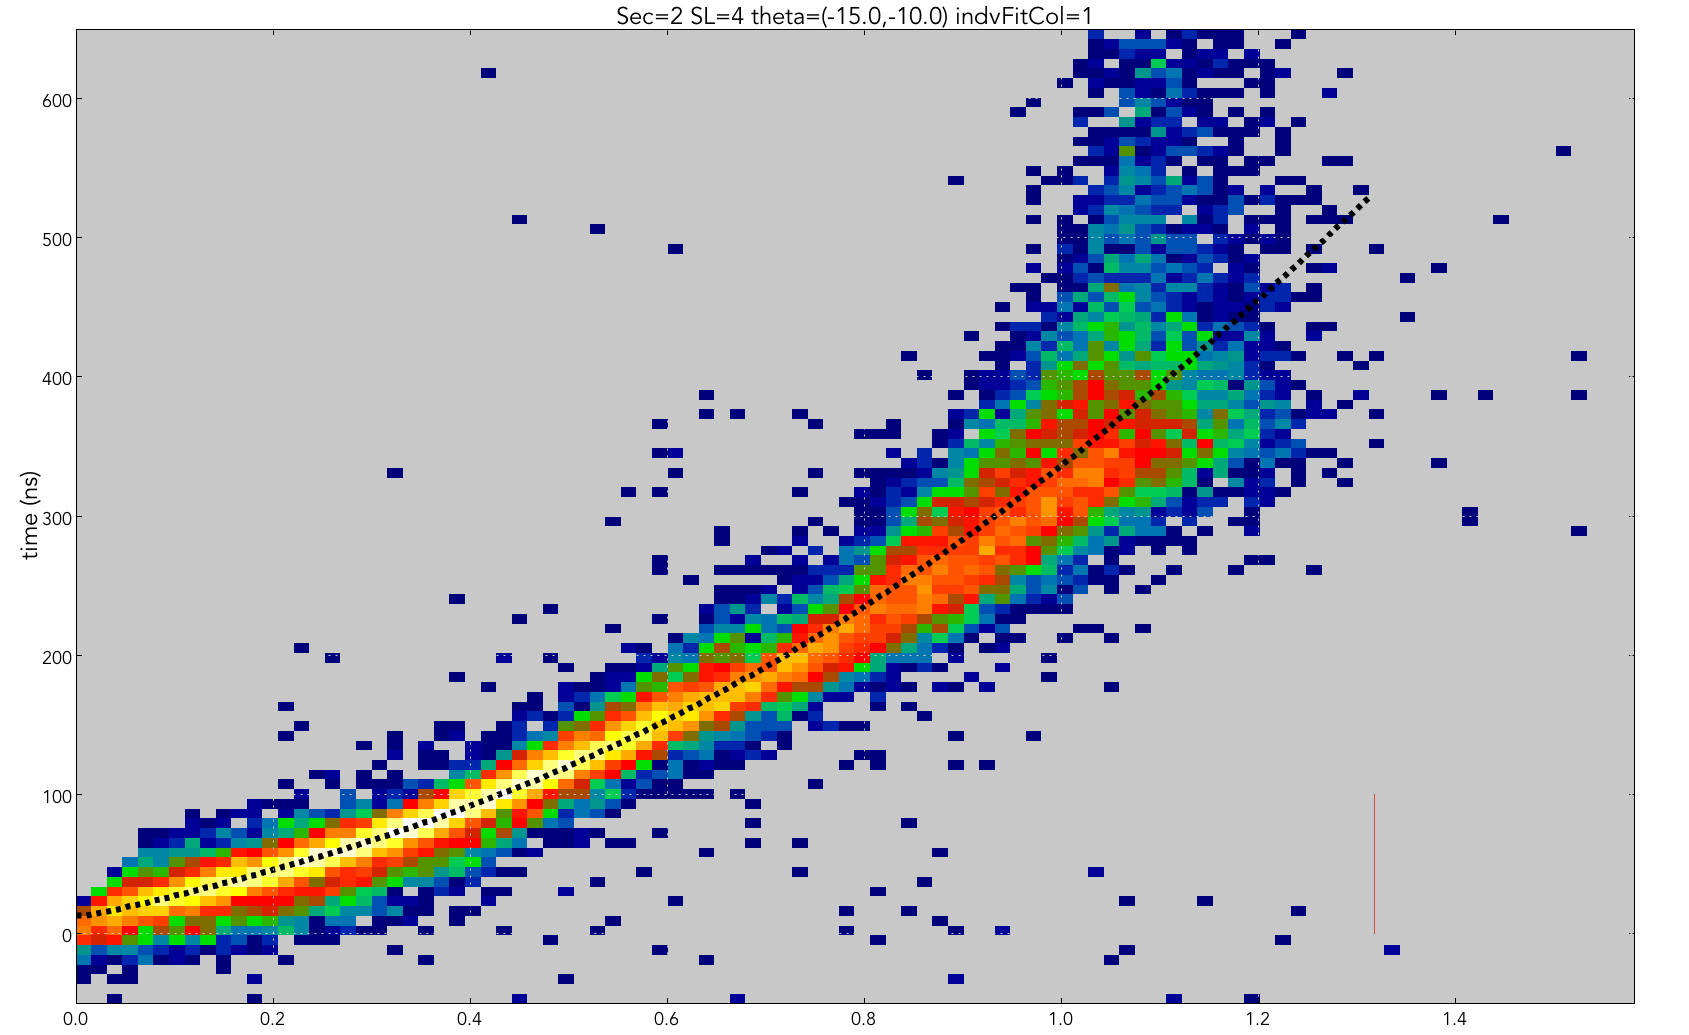
\includegraphics[width=1.0\textwidth]{Figures/time_vs_trkDocaExample_Sec2_SL4_th_m15_m10withFit.png}
    \caption{An example of the time-vs-trkDoca 2D histogram in a given bin (-15,-10) of local angle $\alpha$.}
    \label{fTimeVsTrkDocaWithFit}
\end{figure}


\begin{figure}
    \centering
    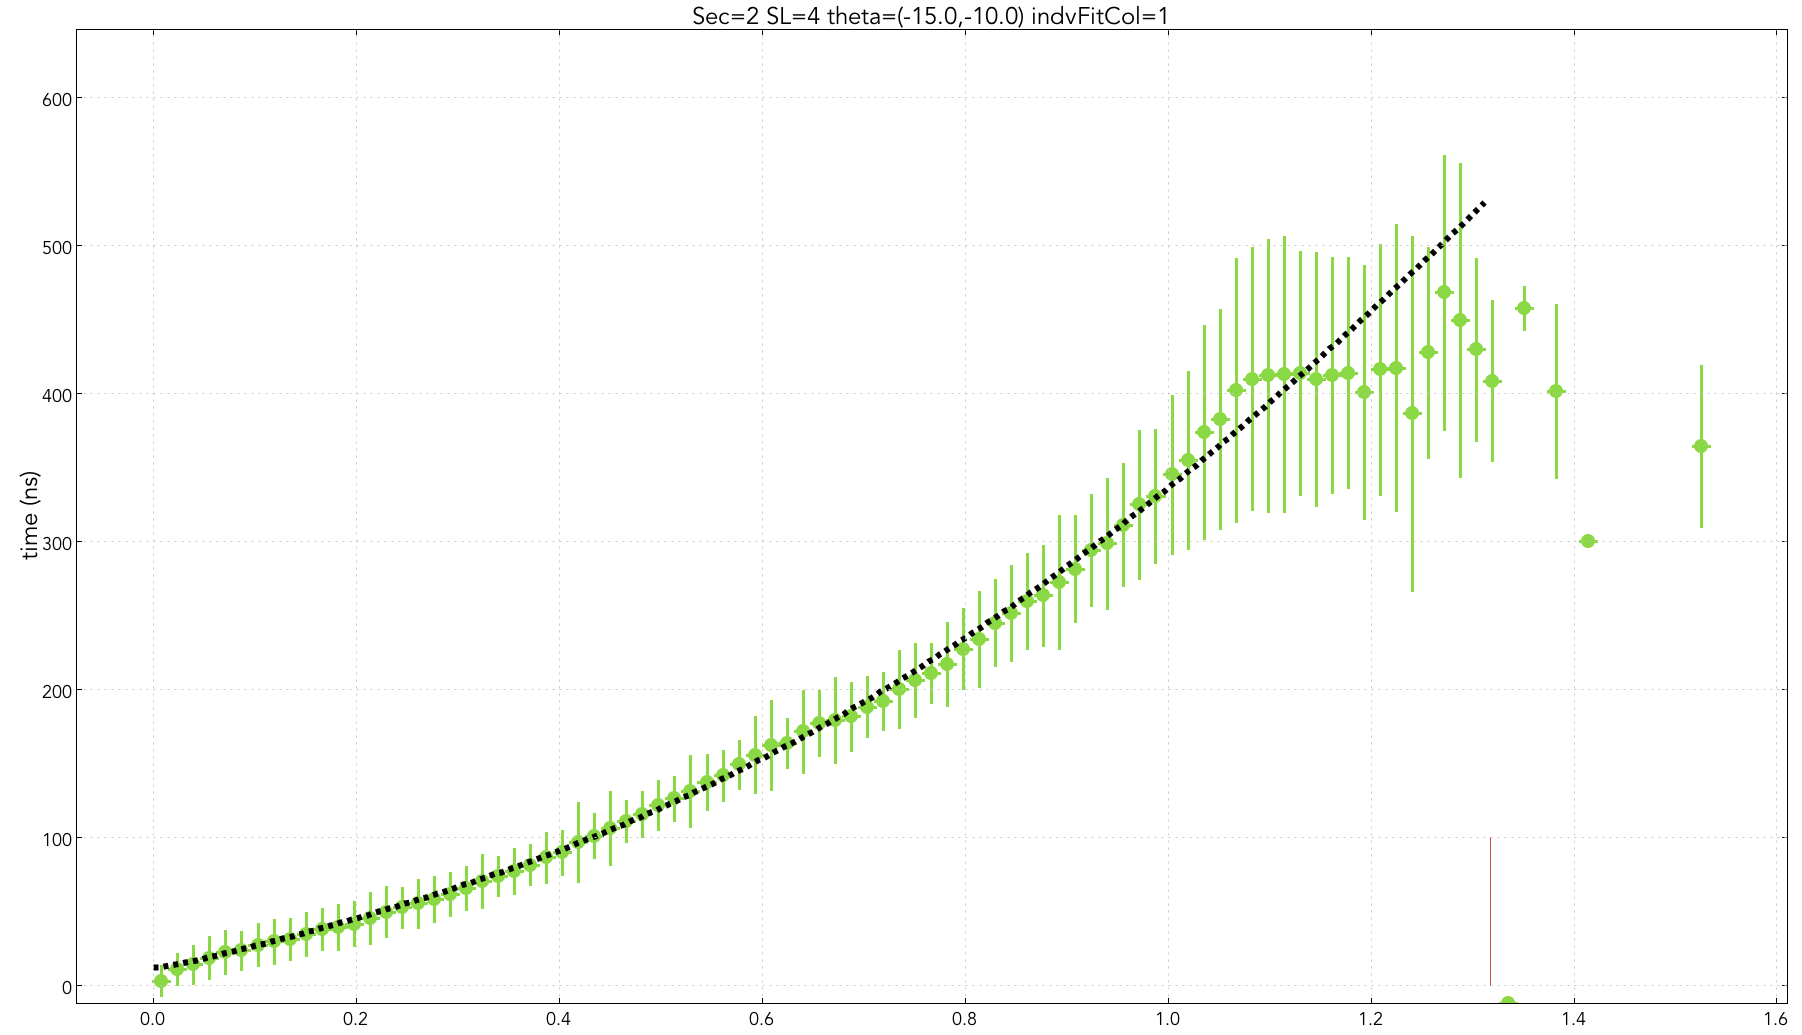
\includegraphics[width=1.0\textwidth]{Figures/time_vs_trkDocaXProfileExample_Sec2_SL4_th_m15_m10withFit.png}
    \caption{An example of the X-profile of  the time-vs-trkDoca 2D histogram in a given bin (-15,-10) of local angle $\alpha$.}
    \label{fTimeVsTrkDocaXProfileWithFit}
\end{figure}



\subsection{Testing the Effect Of Calibration}
When a new iteration of calibration is done, the resulting new values are used to update the CCDB table for the time-to-distance parameters (in the `$dc\_test1$' variation, which is dedicated for use by the DC-calibrators), and the decoded data is reconstructed again (so that the updated value of the parameters are used by the new reconstruction). Once the reconstruction is complete, the distribution of residuals (difference between the trkDoca and calcDoca) for all the good hits are plotted for each sector, region and superlayer (for example, see Figs. \ref{fResidualsDefAllSL} and \ref{fResidualsVsDocaDefAllSL}) and the standard deviations ($\sigma$s) from the corresponding Gaussian fits are compared with the corresponding residuals from the previous iteration of calibration and reconstruction. The residuals provide measures of tracking resolutions of the corresponding drift chambers. It is expected that with new calibrations, the standard deviations of the distributions should get smaller and smaller up to a certain point (after which the resolution will stop being better as we reach the limit of intrinsic resolution of DC). For example, Figs.  \ref{fResidualsDefAllSLiter1} and \ref{fResidualsVsDocaDefAllSLiter1} show improved resolutions after a new iteration of calibration and reconstruction.

\begin{figure}[H]
    \centering
    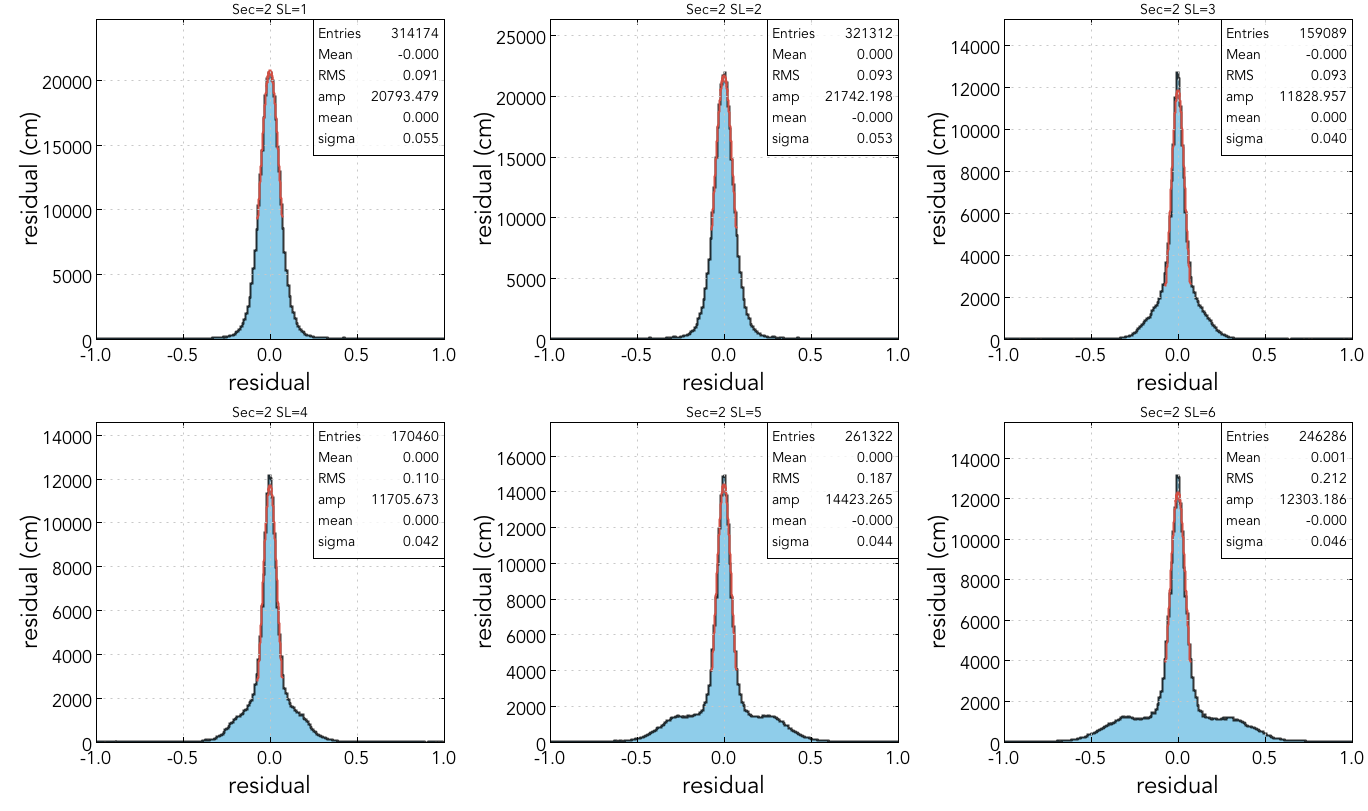
\includegraphics[width=1.0\textwidth]{Figures/residual_defaultT2D_automatedT0.png}
    \caption{Distribution of residuals in the reconstructed data (using nominal or default values of time-to-distance parameters) of KPP run 810.}
    \label{fResidualsDefAllSL}
\end{figure}

\begin{figure}[H]
    \centering
    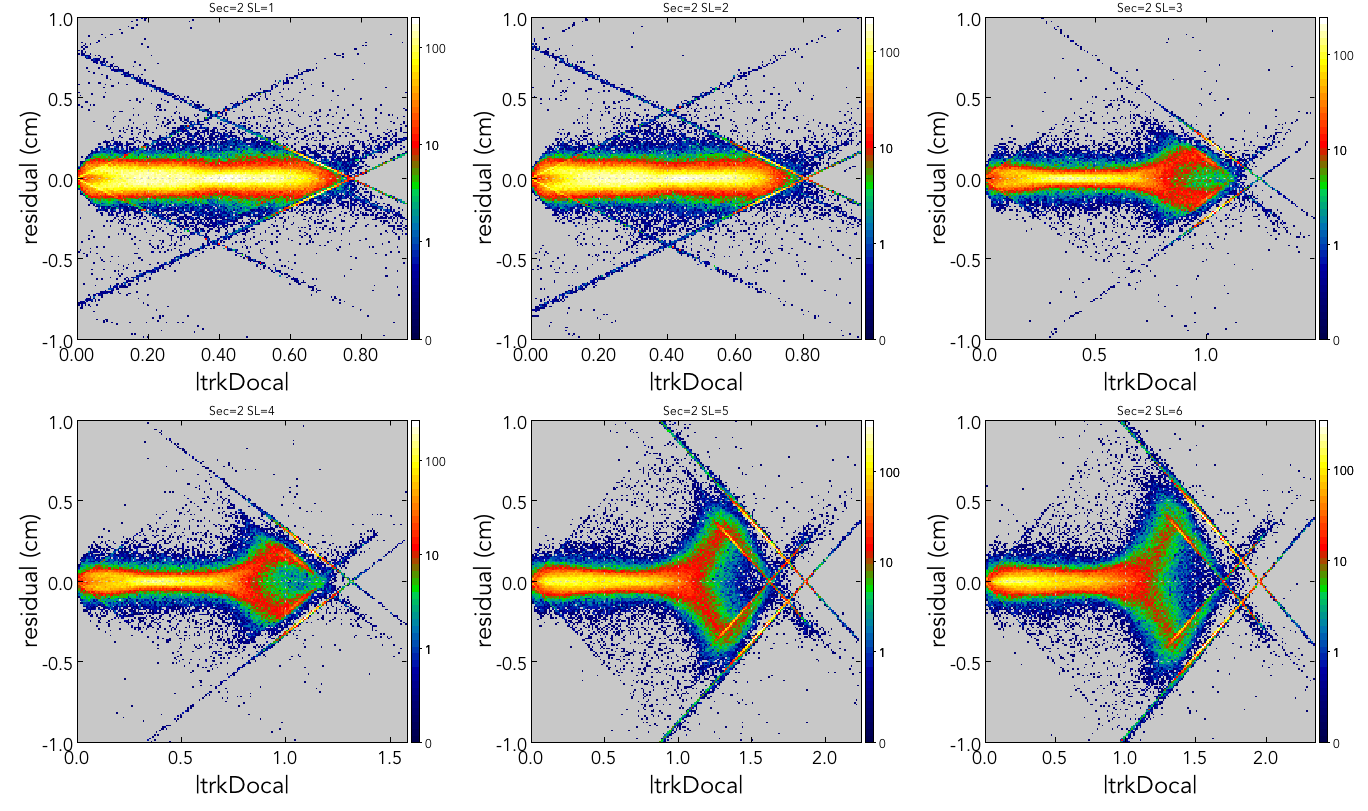
\includegraphics[width=1.0\textwidth]{Figures/residual_vs_trkDoca_defaultT2D_automatedT0.png}
    \caption{Distribution of residuals-vs-trkDoca in the reconstructed data (using nominal or default values of time-to-distance parameters) of KPP run 810.}
    \label{fResidualsVsDocaDefAllSL}
\end{figure}


\begin{figure}[H]
    \centering
    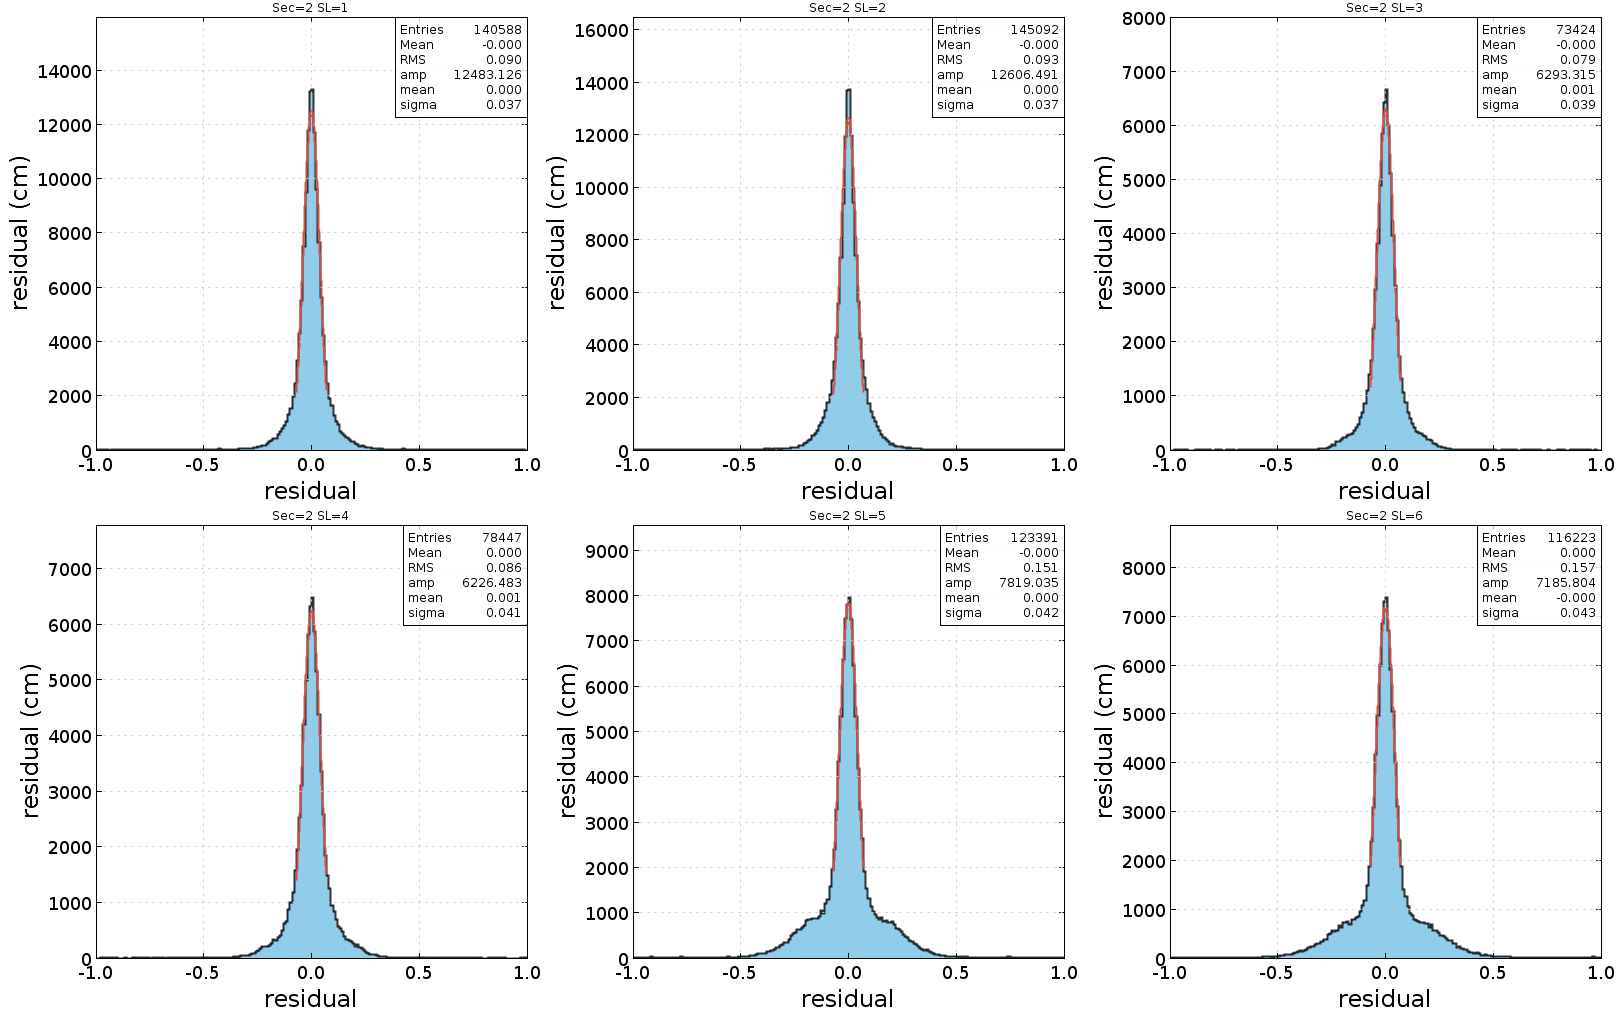
\includegraphics[width=1.0\textwidth]{Figures/residual_Iter2NwDef3T0nw5n.png}
    \caption{Distribution of residuals in the reconstructed data (using new values of time-to-distance parameters obtained from a new iteration of calibration) of KPP run 810.}
    \label{fResidualsDefAllSLiter1}
\end{figure}

\begin{figure}[H]
    \centering
    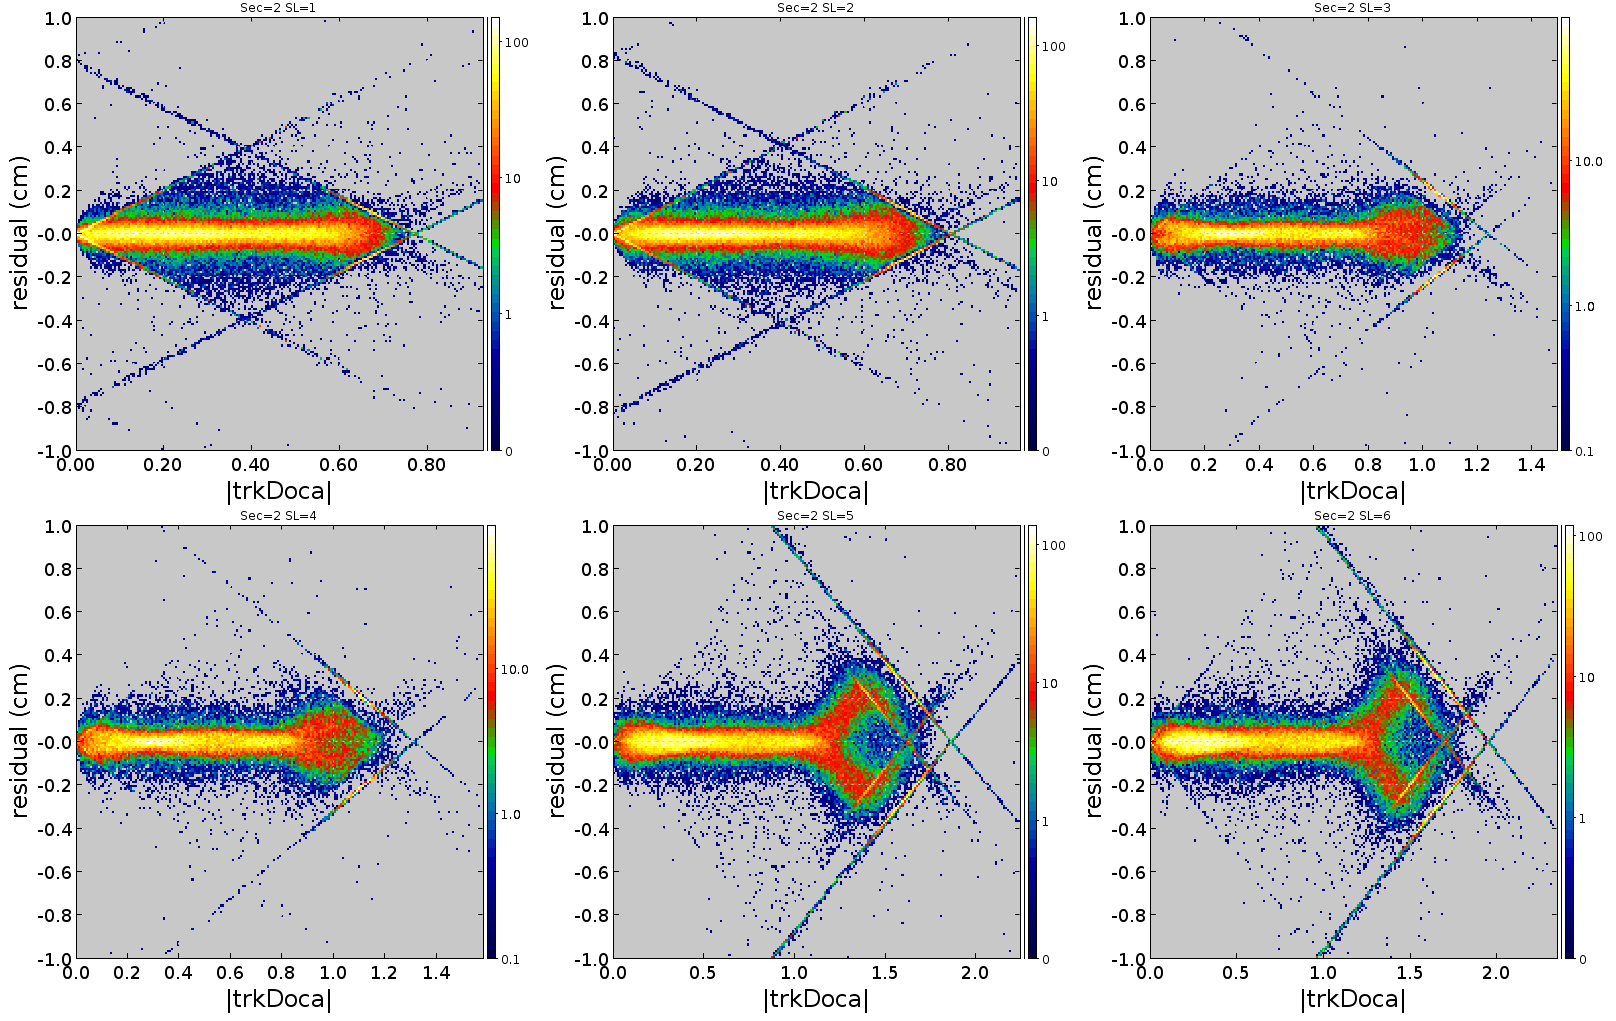
\includegraphics[width=1.0\textwidth]{Figures/residual_vs_doca_Iter2NwDef3T0nw5n.png}
    \caption{Distribution of residuals-vs-trkDoca in the reconstructed data (using new values of time-to-distance parameters obtained from a new iteration of calibration) of KPP run 810.}
    \label{fResidualsVsDocaDefAllSLiter1}
\end{figure}





\section{Graphical User Interfaces (GUI)}
The GUI of the suite consists of a main window that opens up first and then many other windows that open later. 

\subsection{The Main GUI} 
When the program is started, this interface (see Fit. \ref{fMainGUI}) opens up first which allows us to proceed in doing different things. If the T0 correction is not available already, we can click on the `Estimate T0s' button on the top left to start the process for estimating T0s. Although, it's not always practical to reconstruct all data that we want for the calibration, the program also has the capability to run the reconstruction of the decoded data, which can be started by clicking on the 'Run Reconstruction' button. Next, if we already have the reconstructed data that we want to calibrate for the time-to-distance function, we can start doing so by first selecting the one of the two radio buttons (to choose between the linear or non-linear fits to be used), then clicking on the `Choose File' button to select the hipo files with the reconstructed data to be calibrated and finally clicking the `Run Time vs. Distance Fitter' button to start the event loop to read the selected hipo data files and make the histograms that are subsequently used in the fitting procedure. Once the event loop is completed and histograms are all filled, a new GUI pops out which we call Fit Control panel (see Fig. \ref{fFitControlPanel} that allows us to control and constrain our fits. The main gui also has a button at the top that is meant to write to CCDB the results of the calibration (if the program is running in one of the JLab CUE machines - there is no CCDB write access from other machines), although the button hasn't been made to work properly yet as the focus has been more on getting other things right first.

\begin{figure} [H] %[ht]
    \centering
    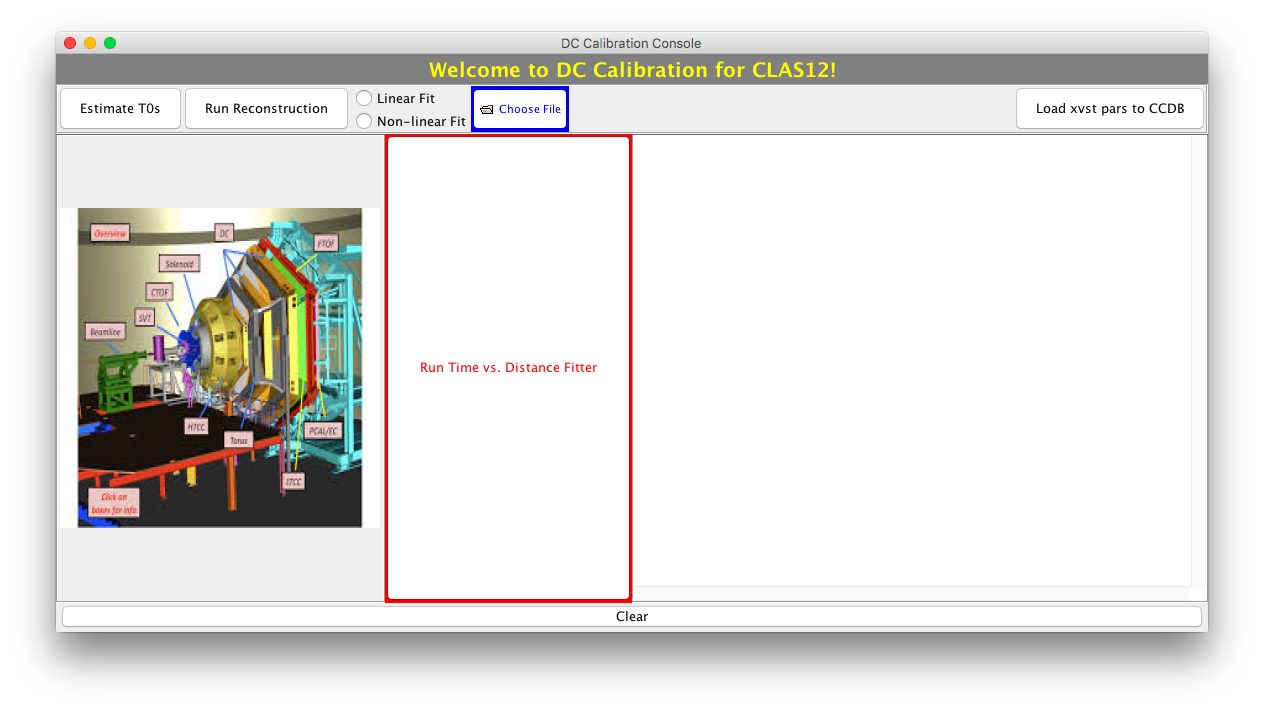
\includegraphics[width=1.0\textwidth]{Figures/Screenshots/screenshotMainGuiDCcalibSuite.png}
    \caption{The current look of the main GUI for the Calibration Suite.}
    \label{fMainGUI}
\end{figure}



\subsection{Fit Control Panel}
\label{ssFitControlPanel}

The fit control panel (see Fig. \ref{fFitControlPanel} for a screenshot of it) which opens up after reading the data files and filling the histograms, has several text fields and buttons to control and monitor the fits as well as a jTextArea where we can see the results of the time-to-ditance fits for a given selection of sector, superlayer and other options. 


\begin{figure} [H] %[ht]
    \centering
    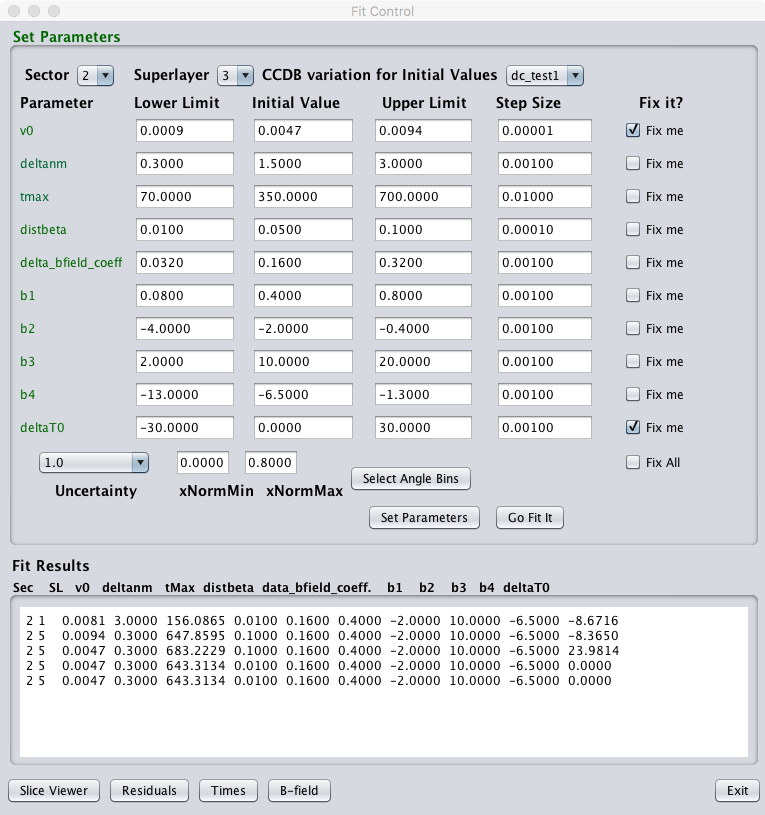
\includegraphics[width=1.0\textwidth]{Figures/Screenshots/screenshotFitControlPanelDCcalibSuite.png}
    \caption{The screenshot of the fit control panel.}
    \label{fFitControlPanel}
\end{figure}

Using the text fields (which by default loads the parameters values from CCDB) we can initialize the values of the fit-parameters, we can give the lower and upper limits to each of them and also we can set the step sizes to be used by the jMinuit during the minimization. Similarly, the check-buttons (labeled `Fix me') on the right allows us to fix the values of the parameters that is set in the Initial Value field. We can fix any number of the parameters. If we fix all the parameters, it wont go through the minimization steps but it will simply create fit lines corresponding to the fit results obtained from the previous iteration and the lines will be drawn and shown on top of the 2D histograms that are used for the calibration. The `Select Angle Bins' button allows us to choose and discard the angle bins to use in the minimization procedure. Clicking this button opens a new window that has as many check buttons as the number of local angle bins and only those bins which are checked will be included in the minimization data set. Finally, we can use the `Go Fit It' button to trigger the fitting and displaying of the results once we set the initial values, limits and check the `Fix me' buttons for the parameters that we want to freeze. Clicking of `Go Fit It' button results in opening a new canvas window (after the calibration fit is completed for the given selection of sector and superlayer etc) that will show the new fits on top of the 2D histograms as well as the corresponding X-profiles (which are shown in different tabs of the new canvas window).


The `Fit-Control' panel also contains other buttons that we can use to monitor various relevant quantities. For example, we can open the `Slice Viewer' (see the next section below), or look at the current resolution (in terms of `residual' and `residual-vs-trkDoca' distributions), various time distributions and B-field distributions by clicking on the corresponding buttons.


\subsection{Slice Viewer}

The slice viewer allows us to investigate the shape of time distributions inside each of the trk-Doca bins (slices), thus allowing us to choose an appropriate function to use to fit to the time distributions and then create the X-profiles. Currently, we're using default method of Gaussian fits in each slice but eventually, we can change that to better alternatives in order to improve the X-profiles.

\begin{figure} [H] %[ht]
    \centering
    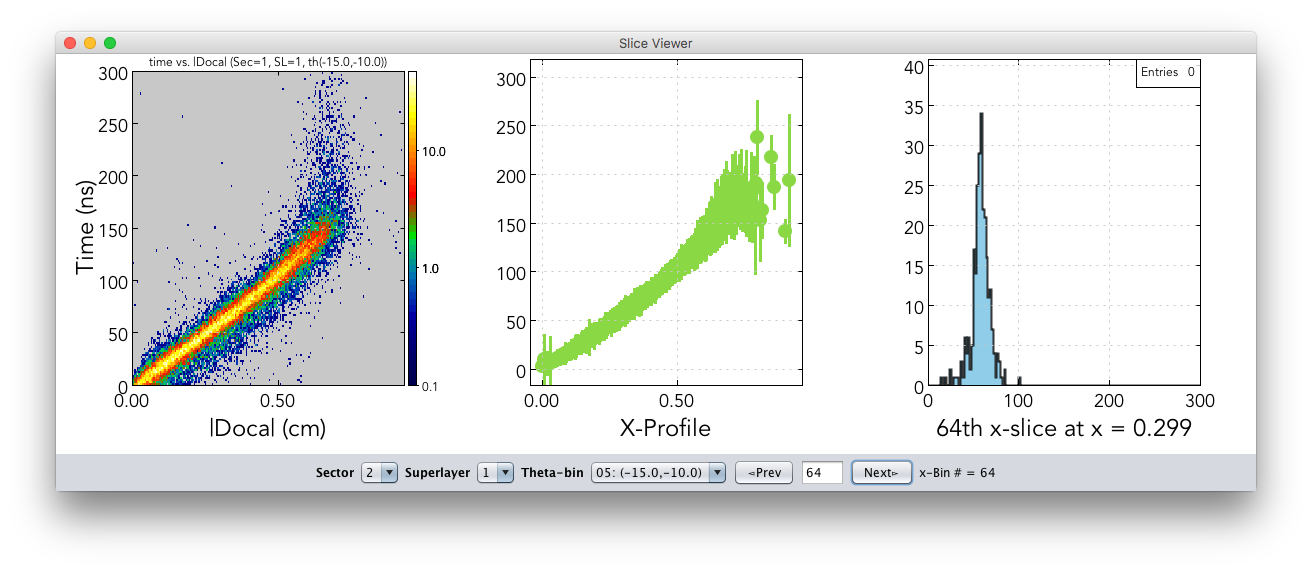
\includegraphics[width=1.0\textwidth]{Figures/Screenshots/screenShotSliceViewer.png}
    \caption{The screenshot of the Slice Viewer window.}
    \label{fSliceViewer}
\end{figure}



% Activate the appendix
% from now on sections are numerated with capital letters
\appendix
\appendixpage
%\addappheadtotoc
% The \appendixpage command adds a separate title “Appendices” above the first appendix, and \addappheadtotoc adds a similar title to the table of contents. These simple modifications cover many people’s needs about appendixes.
% http://www.tex.ac.uk/FAQ-appendix.html


%\section{Propagation Of Uncertainties from fit parameters $p_1$, $p_2$, $p_3$ to T0}






\begin{thebibliography}{9}
  \bibitem{wikiErrProp} Wikipedia, https://en.wikipedia.org/wiki/Propagation\_of\_uncertainty, March, 2017.
%%
%%\bibitem{lamport94}
%%  Leslie Lamport,
%%  \emph{\LaTeX: a document preparation system},
%%  Addison Wesley, Massachusetts,
%%  2nd edition,
%%  1994.
%%
\end{thebibliography}

\end{document}
